\documentclass{article}

\usepackage[francais]{babel}
\usepackage[utf8]{inputenc}
\usepackage[T1]{fontenc}
\usepackage{lipsum}
\usepackage[sc]{mathpazo}
\usepackage{abstract}
\renewcommand{\abstractnamefont}{\normalfont\bfseries}
\renewcommand{\abstracttextfont}{\normalfont\small\itshape}
\linespread{1.05}

\usepackage{microtype}
\usepackage{lmodern}
\usepackage[margin=20mm,top=32mm]{geometry}
\usepackage{multicol}
\usepackage[hang, small,labelfont=bf,up,textfont=it,up]{caption}
\usepackage{booktabs}
\usepackage{float}
\usepackage[hyphens]{url}
\usepackage{hyperref}
\usepackage{lettrine}
\usepackage{paralist}
\usepackage[titletoc,toc,title]{appendix}
\usepackage{graphicx}
\usepackage{alltt}


\usepackage{titlesec}
\renewcommand\thesection{\Roman{section}}
\renewcommand\thesubsection{\Roman{subsection}}
\titleformat{\section}[block]{\LARGE\scshape\centering}{\thesection.}{1em}{}
\titleformat{\subsection}[block]{\large}{\thesubsection.}{1em}{}

\usepackage{fancyhdr}
\usepackage{minted}
\definecolor{LightGray}{gray}{0.9}
\usemintedstyle{monokai}
\pagestyle{fancy}
\fancyhead{}
\fancyfoot{}
\fancyhead[C]{Documentation et modélisation pour les architectures orientée service}
\fancyfoot[RO,LE]{\thepage}

\title{\vspace{-15mm}\fontsize{24pt}{10pt}\selectfont\textbf{Documentation et modélisation pour les architectures orientée service}}

\author{
    \large
    \textsc{Axel Mousset}\\[2mm]
    \normalsize Université de Technologie de Troyes \\
    \vspace{-5mm}
}
\date{Printemps 2016}

%----------------------------------------------------------------------------------------

\begin{document}
    \maketitle

    \begin{abstract}
        Modéliser et documenter un logiciel constituent un travail essentiel pour la maintenance et l'évolution de projet
logiciel sur le long terme. Au delà des document de conception initiaux qui constituent un pré-requis de tout projet
d'ingénierie, un cas extrême de ce besoin de documentation est notamment fourni par le développement de logiciel
open-source qui ajoute la contrainte de rendre disponible le code source et d'ouvrir à la participation d'autres
développeurs au delà de l'équipe projet.

La modélisation UML centrale pour le paradigme objet, les wikis, et frameworks
de test de logiciel sont des ressources importantes pour développer une documentation claire et exploitable. Cependant,
avec le développement d'application logicielless toujours plus complexes et distribuées désormais permises par
l'Internet, aucune stratégie de documentation claire et spécifique n'émerge pour le développement des applications
orientées services.

L'enjeu de ce document est de proposer et de mettre en oeuvre une stratégie de documentation pour la main-
tenance et l'évolution d'applications distribuées et orientées services. Ce travail s'appuiera sur le cas de Buckless,
une application de paiement électronique dématérialisé destinée principalement à la simplification des transactions
dans le cadre des associations étudiantes. Une version majeure de cette solution open source sera bientôt mise en
production par une équipe de développeurs et l'enjeu est de constituer une documentation pertinente pour assurer
la maintenance et l'évolution du projet sur le long terme.

Plusieurs outils sont considérés (modèles UML, outils de documentation d'API, wiki) afin de documenter les
aspects statiques, les principales interfaces et dépendances, et les aspects comportementaux du système. A partir
de l'exemple d'autres cas de projets open-source, une stratégie de documentation sera ainsi formalisée et mise en
oeuvre. Cette dernière est mise à l'épreuve en interrogeant son utilité lors de l'ajout de nouveaux composants et
fonctionnalité au projet Buckless.
    \end{abstract}

    \newpage
    \tableofcontents

    \thispagestyle{fancy}

    \newpage
    \section{Etat de l'art}
        Alors qu'un état de l'art classique se vaut éxhaustif, cette partie place volontairement un filtre sur
les éléments proposés. En effet, la diversité des outils est telle que seuls ceux poussés de
l'avant par la communauté de développeurs seront abordés.
D'autres outils moins populaires (comme les diagrammes UML de composants), mais témoignant d'une pertinence
particulière pour les architectures orientées services, seront également étudiés.

\subsection{Documentation du code}
    \subsubsection{Commentaires}
La documentation du code source au travers de commentaires est probablement l'étape la plus
importante dans un projet faisant appel à une équipe de plusieurs développeurs.
Certaines bonnes pratiques se sont démarquées avec le temps, jusqu'à créer une formalisation de
ces commentaires, qui donnera plus tard la célèbre \textbf{JavaDoc} pour le language Java.
Ce standard est décliné pour la plupart des languages de programmation : on retrouve ainsi
jsDoc pour javascript, doxygen pour C/C++, etc..

\begin{listing}[ht]
    \begin{minted}[
        bgcolor=black,
        fontsize=\footnotesize
    ]{javascript}
    /**
     * Create an array of all the right files in the source dir
     * @param      {String}   source path
     * @param      {Object}   options
     * @param      {Function} callback
     * @jsFiddle   A jsFiddle embed URL
     * @return     {Array} an array of string path
     */
    function collectFiles(source, options, callback) {
        foo()
    }
    \end{minted}
    \caption{Exemple de documentation de fonction avec jsDoc}
\end{listing}

Au delà de l'intérêt immédiat des commentaires sur la lecture du code, ce formalisme vient avec
un ensemble d'outil permettant l'extraction des commentaires, puis la génération d'une documentation
statique de la structure du code.

\begin{figure}[ht]
    \centering
    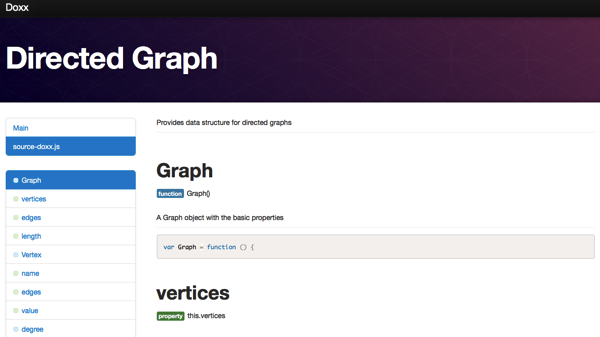
\includegraphics[scale=0.5]{./assets/doxx.png}
    \caption{Une documentation HTML génerée par Doxx et jsDoc}
\end{figure}

On voit donc que les formalismes de commentaires de code sont une première étape essentielle
à la documentation d'un projet logiciel. Ces documentations sont cependant sous forme de texte.
Ainsi, sur des sources de plusieurs centaines de fonctions / classes, il peut être intéressant de
proposer une vue d'ensemble du code. C'est dans cette optique que nous allons étudier l'utilisation
des diagrammes UML de classe.

    \subsubsection{UML - Diagrammes de classe}
UML\footnote{Unified Modeling Language} est un language de description, né de collaboration
de la communauté orienté-objet, devenu un standard dans la description de systèmes (informatiques ou non).
Ses spécifications décrivent un grand nombre de diagrammes. Parmis les plus poluaires, le diagramme
de classe pour la modélisation orientée-objet. De plus, le paradigme orienté-objet étant
quasiemment systématiquement utilisé dans le développement logiciel moderne, il parait naturel
de le présenter ici.

\begin{figure}[ht]
    \centering
    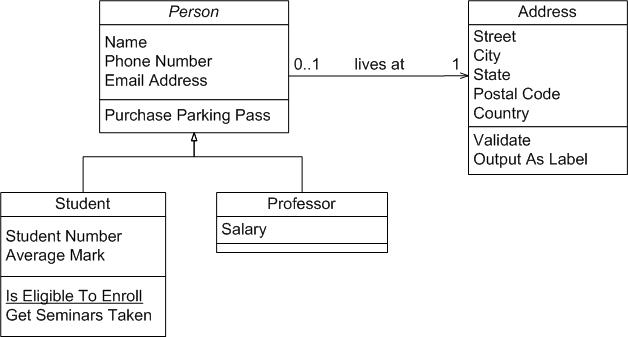
\includegraphics[scale=0.7]{./assets/class.jpg}
    \caption{Un diagramme de classe.}
\end{figure}

Le diagramme de classe peut être utilisé en amont comme outil de réflexion sur la structure
d'un projet logiciel. Lors de la production du code, cette structure est amenée à être alterée.
Ainsi, une deuxième utilisation émerge, celle de la description de la structure à un instant du code
a un instant t.
Il existe plusieurs logiciels permettant d'adopter cette "démarche inverse", à savoir pouvoir
produire des diagrammes à partir de code existant.

Cette utilisation est d'autant plus intéressante qu'elle permet aux côtés des documentations
statiques vues précédemments, de rendre compte de l'état du code à travers différents
canaux (textes, visuels..). De plus, contrairement au formalismes de documentation par commentaire,
la syntaxe UML des diagrammes de classes permet de visualiser de manière intuitive la nature des
liens entre les différentes entités.

\newpage
\subsection{Documentation de service}
À l'image de la documentation normalisée visant à rendre le code accessible à d'autres développeurs,
le besoin de décrire des WebServices est vite apparu. Nous allons présenter ici les trois formalismes
de description d'API REST les plus populaires.

    \subsubsection{Swagger}
        \paragraph{}
            Swagger est le premier éssai de formalisme de description d'API REST. Son but, définir un
            standard \textit{language-agnostic}\footnote{Qui ne dépend pas du language de programmation}
            permettant aux humains comme à des outils informatiques d'explorer une API sans avoir à
            plonger dans le code. \label{swaggerdef} Ses créateurs définissent Swagger\cite{Swagger} par analogie comme
            l'équivalent des interfaces en programmation orienté-objet, appliqué aux services.

        \begin{listing}[ht]
            \inputminted[
                bgcolor=black,
                fontsize=\footnotesize
            ]{YAML}{./assets/swagger-petstore.yml}
            \caption{Exemple de définition d'API Swagger}
        \end{listing}

        \paragraph{}
            L'ensemble des outils dérivés incluent : un générateur de code client / serveur, un éditeur
            de définition en ligne, et un générateur de documentation dynamique.
            La génération de documentation dynamique passe tout d'abord par la description du service
            par le formalisme de Swagger. Cette description s'est fait avec le language de description YAML
            \footnote{Superset de JSON en plus lisible}, ou JSON.

        \begin{figure}[ht]
            \centering
            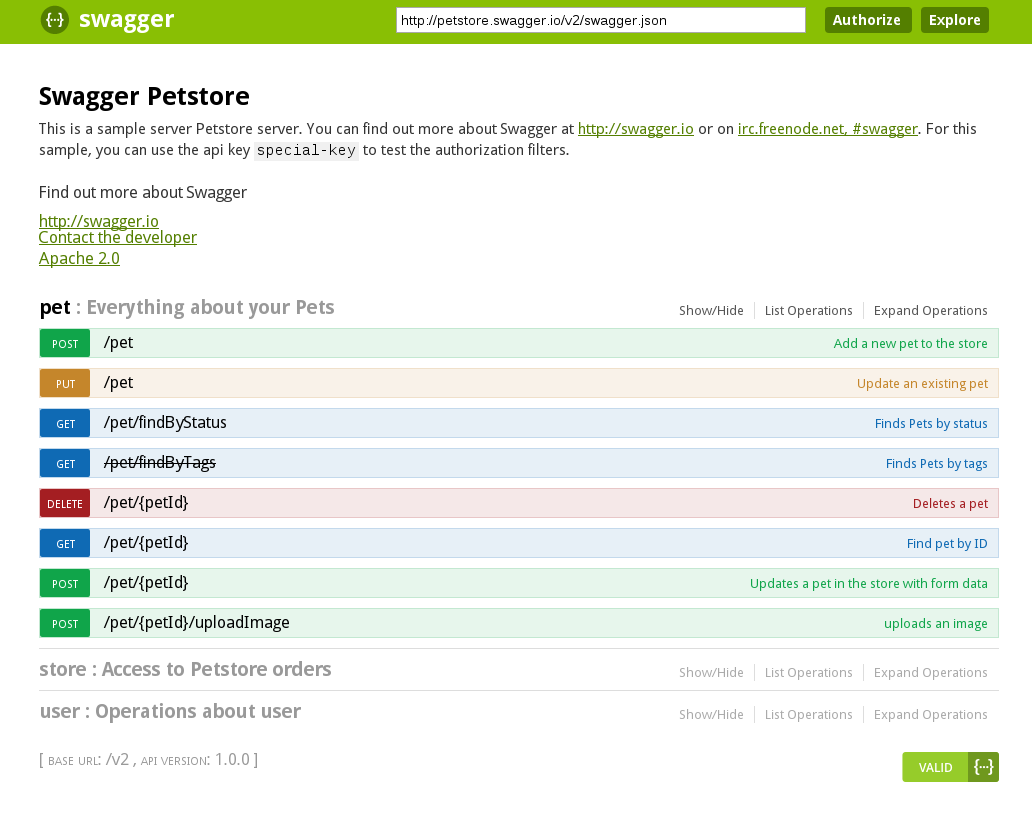
\includegraphics[scale=0.4]{./assets/swagger.png}
            \caption{Documentation dynamique générée par Swagger}
        \end{figure}

    De nombreuses alternatives à Swagger existent : RAML, Apiary, API blueprint... Elles reposent
    globalement sur les même concepts, il n'est pas pertinent de détailler leur spécificités ici.

\newpage
\subsection{Documentation de système}
    \subsubsection{Wiki}
        Un wiki est une application web qui permet de la gestion collaborative de contenu.
        Sa structure flexible permet de pouvoir centraliser, trier et distribuer les différentes strates
        de documentations discutées ci-dessus. De plus, il peut servir pour ajouter du contenu décrivant
        le système et ce qui gravite autour, à un niveau de description qui n'avait pas sa place dans les
        contextes vu précédemment. Un rassemblement des wiki les mieux tenus dans le millieu de l'open source
        est proposé par GitHub\cite{wiki}.

        \begin{figure}[ht]
            \centering
            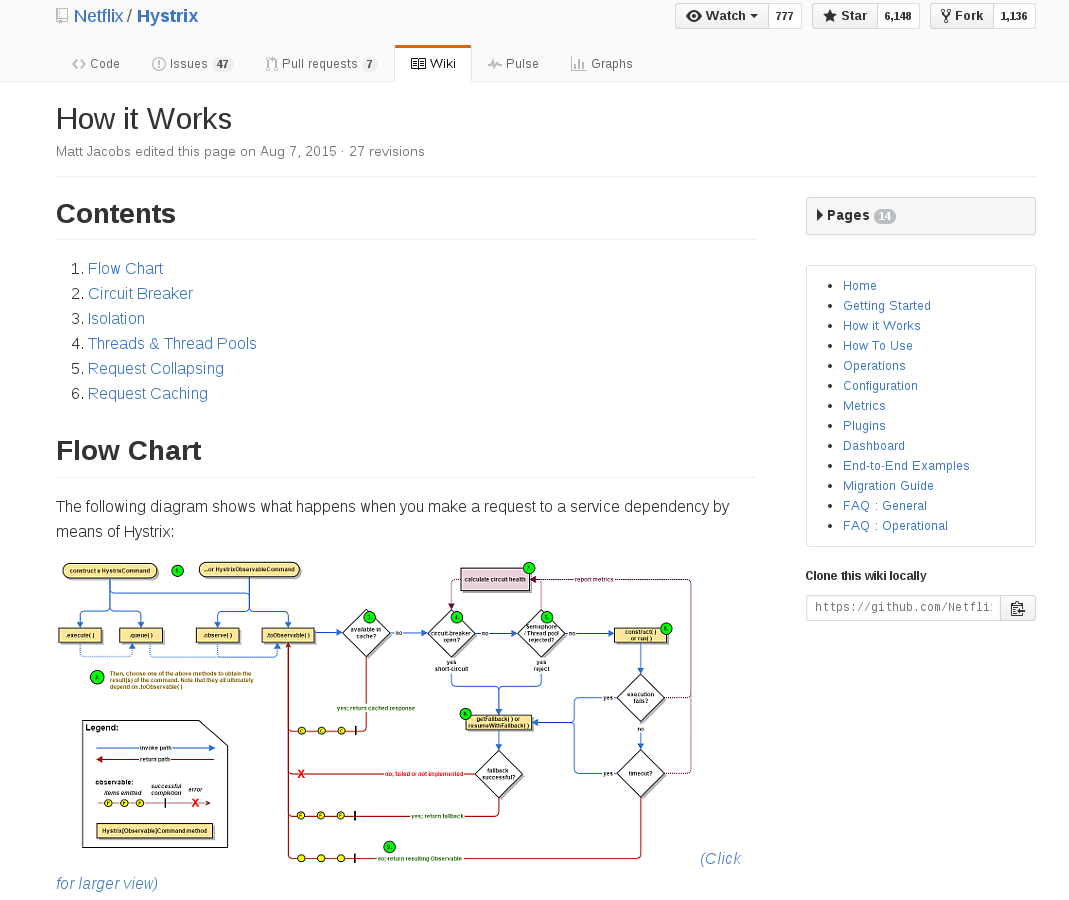
\includegraphics[width=\textwidth]{./assets/wiki_example.png}
            \caption{Un exemple de wiki alliant plusieurs moyens de documentations}
        \end{figure}

\newpage
\subsection{Intégration dans les processus de développement}
        Une grande problématique du développement logiciel est la maintenance de la documentation associée
        à jour. Nous allons étudiers les différents levier qui permettent d'intégrer la documentation
        à la production de code.

    \subsubsection{Modélisation avant production}
        La première étape avant la production du code est de spécifier et modéliser les systèmes et leurs
        interactions. On pourra alors commencer par modéliser les ressources : diagrammes de classes,
        diagrammes entité / association. Vient ensuite la description des services avec des diagrmames de composants
        et des outils type Swagger, RAML, etc. Au moment de la production du code, et durant toute son évolution,
        l'intégration de la documentation s'appuiera sur un outil incontournable, le linter.

    \subsubsection{Linters}
        Un linter désigne un logiciel d'analyse statique de code. Configuré pour, un linter peut vérifier
        la présence de commentaires de type javadoc. On utilisera cette fonctionnalité de vérification
        pour intégrer la documentation au développement logiciel.

        \begin{figure}[ht]
            \centering
            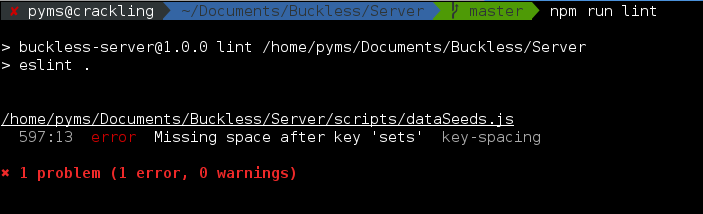
\includegraphics[width=\textwidth]{./assets/eslint.png}
            \caption{Exemple de sortie d'eslint}
        \end{figure}

        Pour ce qui est de la maintenance à jour des diagrammes UML, certains outils proposent de générer
        les diagrammes à partir du code. Cependant les résultats ne sont pas toujours satisfaisant, on
        ne les présentera donc pas ici.

    \subsubsection{Git hooks}
        \paragraph{}
            \label{hooks}
            Git est aujourd'hui l'outil de versionning de code le plus largement utilisé. Parmis ses possibilité,
            celle de définir des hooks\footnote{Action déclenchée automatiquement} lorsqu'une nouvelle version est propagée.
            Ainsi, il est possible d'utiliser le linter de code en avec un hook "pré-commit", c'est à dire avant la
            propagation d'une nouvelle version, pour n'autoriser la propagation qu'une fois que le linter valide l'état du code et
            de ses commentaires.\\
            Cette méthode est néanmoins un peu brutale, car parfois incompatible avec certaines méthodes
            de développement. Il est parfois critique de devoir déployer sur la production un bugfix,
            ce qui peut être gênant lorsque l'ont travaille avec des hooks qui ne sont pas forcémment triviaux à désactiver.\\
            Elle n'est cependant pas à oublier : certaines grosses entreprises avec des exigences de
            qualité de code très strictes utilisent des mécanismes similaires.


        \paragraph{}
            Pour créer un hook de pré-commit, il faut créer un fichier qui contient des instructions bash,
            qui sera executé avant chaque commit. En cas d'erreur, le commit n'est pas effectué.

            \begin{minted}[bgcolor=black,formatcom=\color{white}]{bash}
touch .git/hooks/pre-commit
            \end{minted}

            Ce fichier doit avoir les droits d'execution :

            \begin{minted}[bgcolor=black,formatcom=\color{white}]{bash}
chmod +x .git/hooks/pre-commit
            \end{minted}

            Enfin, il ne reste plus qu'à appeler le linter :

            \begin{listing}[ht]
                \begin{minted}[bgcolor=black,formatcom=\color{white}]{bash}
#!/bin/sh

eslint .
                \end{minted}
                \caption{Exemple de script de hook}
            \end{listing}

            Ainsi, lors de l'appel d'un commit, avec un code non conforme, on obtient la figure suivante.

            \begin{figure}[ht]
                \centering
                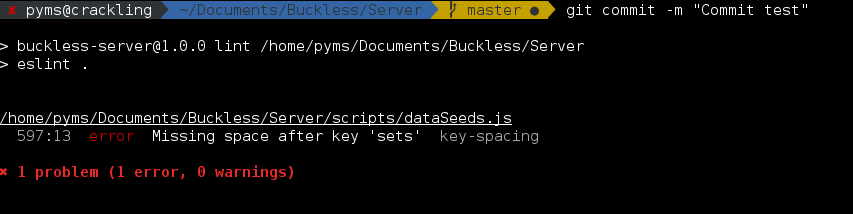
\includegraphics[width=\textwidth]{./assets/hook.png}
                \caption{Resultat du hook : le commit est annulé}
            \end{figure}

    \subsubsection{Intégration continue}
        L'intégration continue désigne un ensemble de pratiques utilisées en génie logiciel consistant
        à vérifier à chaque modification de code source que le résultat des modifications ne produit
        pas de régression dans l'application développée. Il assure la bonne compilation du code,
        mais aussi le jeu des tests unitaires, le packaging, le déploiement et l’exécution des tests
        dans un environnement d’intégration. Intégrer le lint au coeur de ce processus permet
        de déclarer le code «non saint», et ainsi pousser le développement à se faire en même
        temps que celui de sa documentation. Parmis les outils d'intégration continue les plus
        populaires, on pourra citer : Travis CI, Circle CI, Jenkins, Gitlab CI. L'écosystème est cependant
        en pleine évolution, et il existe des dizaines d'alternatives.

    \subsubsection{Déploiement continu}
        On appelle déploiement ocntinu le fait d'automatiser les mécanismes de déploiement du code en
        production à la suite de l'intégration continue. Un cas d'utilisation immédiat pour la documentation
        est alors la mise en ligne automatique des documentations générées par Doxx ou Swagger après
        chaque nouvelle version du code. Cette pratique est d'autant plus facile d'accès maintenant que
        GitHub propose d'héberger des sites statiques gratuitement pour les projets open-source.

    \newpage
    \section{Cas d'études open-source}
        Avant de définir une stratégie de documentation pour le projet Buckless, nous allons
nous intéresser à la manière dont les différents outils présentés précédemment ont été
intégrés par de gros projets open source.\\
Ces projets ont été choisis pour leur similitude avec le projet Buckless, que ce soit
par les technologies utilisées, le type de logiciel produit, l'architecture logicielle
semblable, etc.

\subsection{Nylas N1}
    \subsubsection{Présentation}
        Nylas est une organisation réalisant le projet N1, un client mail se basant sur des technologies web.
        En effet, le projet utilise un chromium\footnote{Navigateur web} embarqué  pour distribuer une application
        web en tant qu'application native. Cela permet d'avoir une interface facilement stylisable et extensible,
        en plus d'être multiplateforme et portable.\\
        Cette interface utilise une API REST, ouverte, dont la documentation est générée à partir du code.
        Malheureusement, le code source de cette API n'est pas disponible et il n'y a pas moyen de connaître la méthode de génération.
        On peut toutefois observer que la génération de la documentation est faite en interne via un script,
        et non automatiquement à l'aide d'intégration continue.

    \subsubsection{Stratégie de documentation}
        \paragraph{}
            Une documentation est aussi disponible pour l'application en elle-même.
            Vu que le projet est basé sur le paradigme de Programation Orienté Objet, les classes sont assez facile à identifier avec "l'API Reference".
            De plus, N1 utilise les Web Components — qui apportent la modularité aux sites webs en découpant chaque partie en composants autonomes,
            et ils sont eux aussi facilement identifiables.

        \begin{figure}[ht]
            \centering
            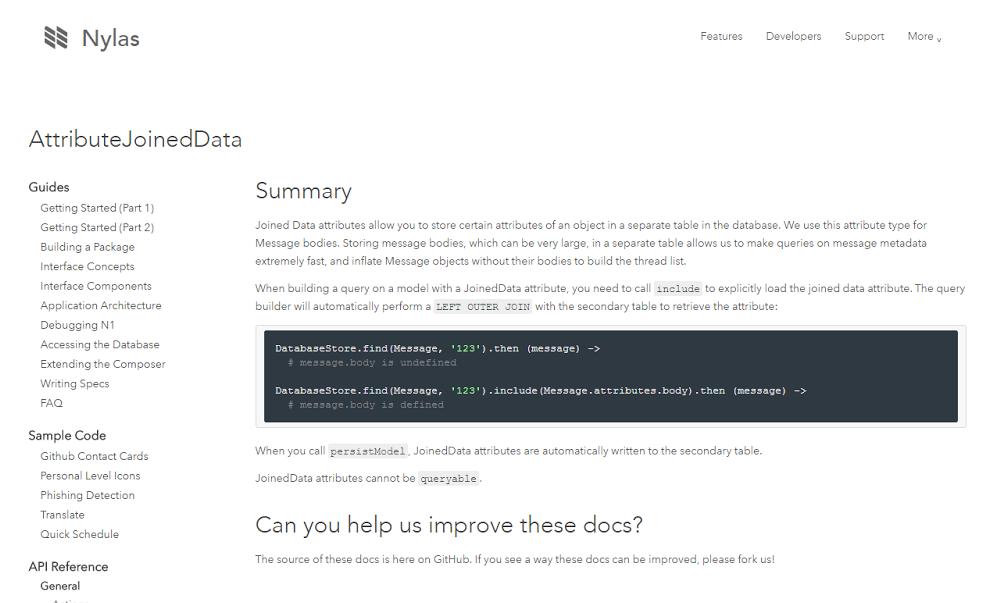
\includegraphics[scale=0.35]{./assets/nylasdoc2.png}
            \caption{Acceuil de la documenation}
        \end{figure}

        \paragraph{}
            L'intérêt majeur de cette documentation est qu'elle est générée via le code source de l'application.
            En utilisant les commentaires, leur script de génération de documentation va créer une arbre syntaxique (AST\footnote{Abstract Syntax Tree}),
            aussi utilisé dans la compilation de programmes.

        \begin{figure}[h]
            \centering
            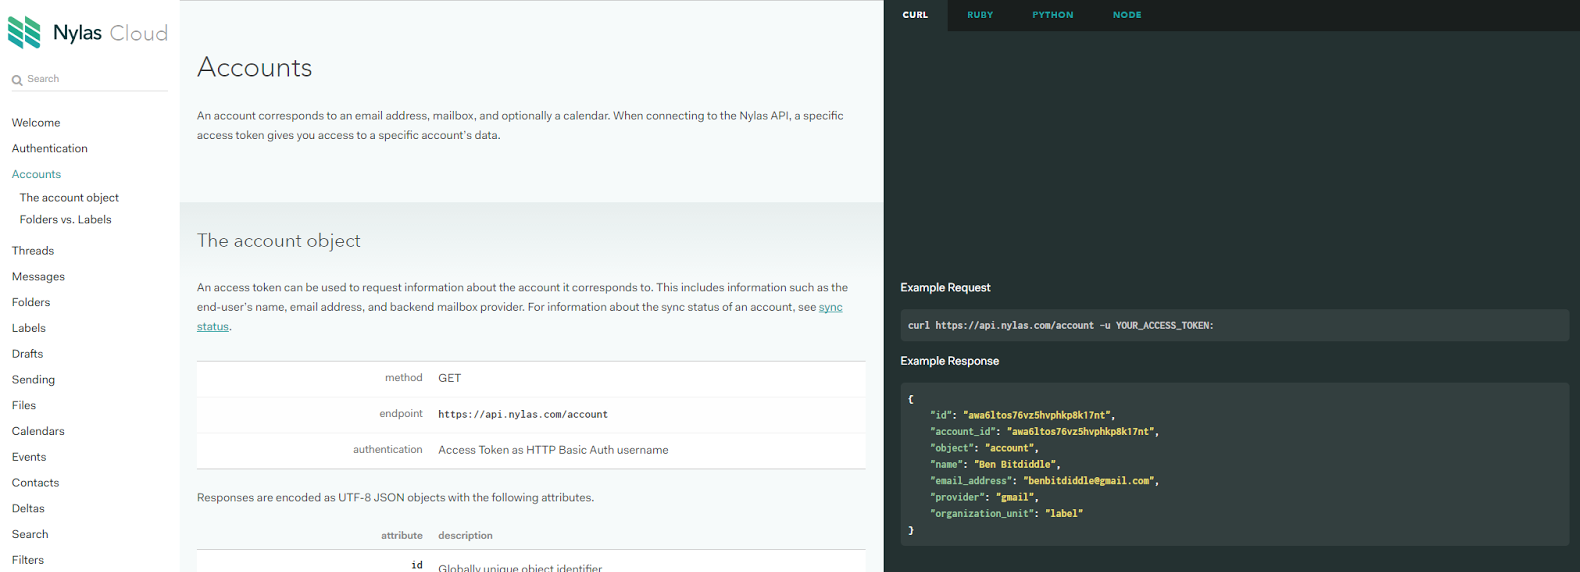
\includegraphics[width=\textwidth]{./assets/nylasdoc.png}
            \caption{La référence de l'API}
        \end{figure}

        \begin{listing}[ht]
            \begin{minted}[
                bgcolor=black,
                fontsize=\footnotesize
            ]{ruby}
# Public: A mutable text container with undo/redo support
class TextBuffer
  @prop2: "bar"

  # Public: Takes an argument and does some stuff.
  #
  # a - A {String}
  # Returns {Boolean}.
  @method2: (a) ->
            \end{minted}
            \caption{Exemple de commentaire TomDoc}
        \end{listing}

        \paragraph{}
            Au niveau des commentaires, un dérivé de jsDoc (TomDoc\cite{tomdoc}) est utilisé, plus adapté
            pour des grosses parties de documentation (là où jsDoc est plus adapté pour l'auto complétion et la documentation rapide).
            La génération de l'AST est faite à l'aide d'une librairie spécialisée\cite{donna}.
        \begin{listing}[ht]
            \begin{minted}[
                bgcolor=black,
                fontsize=\footnotesize
            ]{json}
"files": {
"spec/metadata_templates/classes/class_with_prototype_properties.coffee": {
  "objects": [
        "type": "class",
        "name": "TextBuffer",
        "bindingType": null,
        "classProperties": [],
        "prototypeProperties": [11, 11],
        "doc": " Public: A mutable text container with undo/redo support\n\n "
[...]
            \end{minted} \caption{Une partie de l'AST produit sous forme de JSON}
        \end{listing}

        \paragraph{}
            L'AST généré est ensuite transformé en code quasiment exportable en HTML, en utilisant une deuxième librairie\cite{tello}.
            Enfin, Nylas possède un script qui va automatiquement réaliser l'AST puis le contenu et générer le code HTML de la documentation.
            Le code est ensuité publié sur une branche spécifique à la documentation de leur projet.
            Cette branche est automatiquement mise en ligne par GitHub\cite{ghpages} ce qui permet uniquement en
            modifiant le code, de mettre à jour la documentation en ligne directement.

\subsection{Ghost}
    \subsubsection{Présentation}
        L'idée de Ghost est née lorsque Jon O'Nolan, fondateur de Wordpress, se rendit compte que
        Wordpress était devenu beaucoup trop complexe pour une simple plateforme de blogging. C'est
        à partir de ce constat qu'il décida de créer une plateforme de blogging dédiée uniquement au
        contenu. Débutant de projet de zéro, Ghost a été construit sur du javascript côté client et
        serveur.\\
        Ajourd'hui, Ghost est une plateforme massivement utilisée. C'est d'ailleurs un projet open-source,
        qui base son modèle économique sur du Software As A Service (SAAS). C'est donc autant pour les
        similitudes technologiques que celles du business model que Ghost a été retenu en tant qu'exemple.

    \subsubsection{Stratégie de documentation}
        \paragraph{}
            Contrairement à Nylas N1, Ghost a pris le partie de ne pas intégrer la documentation à sons processus
            de développement. La documentation est quelque chose de complètement indépendant du code,
            et possède son propre versionning. Ghost propose deux grands types de documentation : une documentation
            orientée utilisateur, et une orientée développeur. C'est sur cette dernière que va se concentrer
            notre analyse.

        \begin{figure}[h]
            \centering
            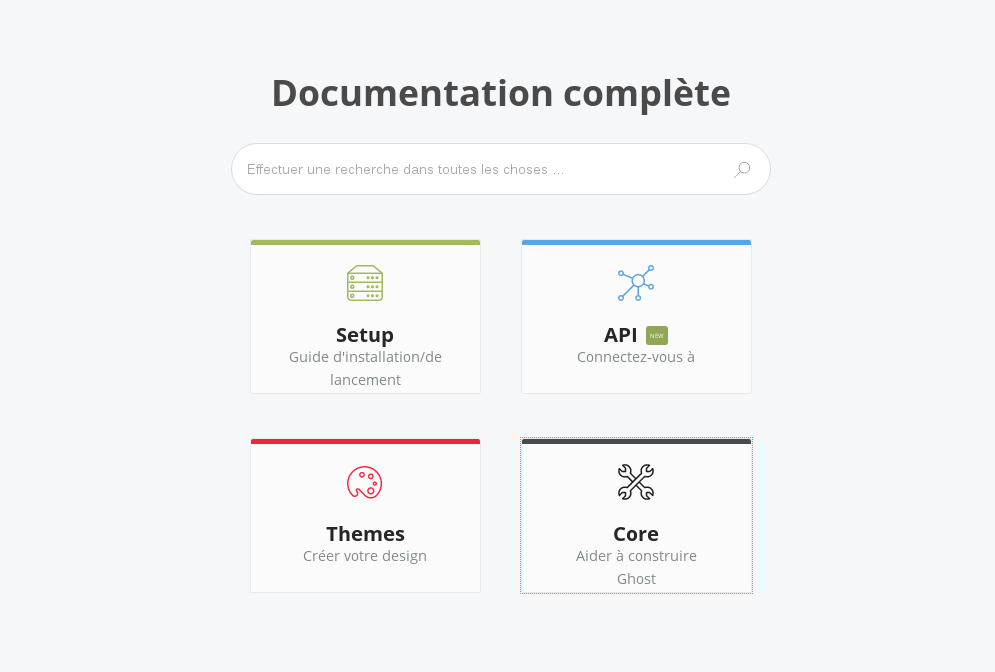
\includegraphics[scale=0.35]{./assets/ghost1.png}
            \caption{Acceuil de la documenation}
        \end{figure}

        \newpage
        \begin{figure}[h]
            \centering
            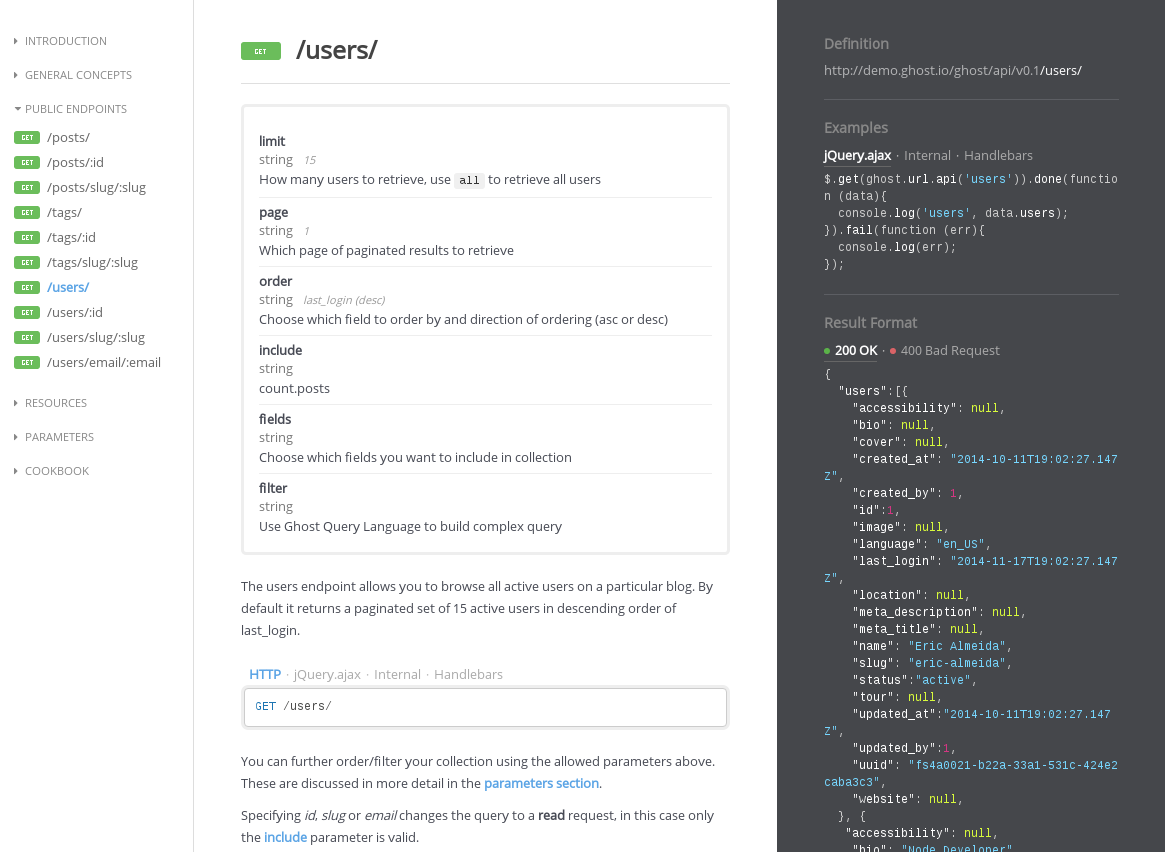
\includegraphics[height=12cm]{./assets/ghost2.png}
            \caption{API Reference}
        \end{figure}
        \paragraph{}
            Parmi la documentation développeur, deux grands axes sont développés.
            Le premier, est une documentation de l'API RESTful de Ghost. Un formalisme de description
            d'API tel que Swagger (probablement API Blueprint) est utilisé pour générer une documentation
            dynamique. Il n'est malheureusement pas possible d'en avoir la certitude, puisque la solution
            \footnote{readme.io} utilisée est payante.



        \newpage
        \paragraph{}
            Le deuxième est une documentation de la structure interne du serveur. Celle-ci aborde moins
            le côté "fonctionnel" du serveur, à savoir les différentes routes et ce qu'elles retournent, mais
            plus une approche structurelle qui permet de former les potentiels contributeurs. Elle
            décrit notemment le style de code à utiliser lors d'une contribution, l'architecture globale
            de l'application et ses composants, mais aussi des indications quant au déploiement de Ghost.
            Cette documentation se présente sous la forme d'un Wiki, hébergé directement sur le
            dépôt du projet sur GitHub. Différents types de documents sont proposés : du texte, des
            diagrammes et des schémas ASCII. On peut remarquer qu'ucun formalisme n'est utilisé
            pour les différents diagrammes.

        \begin{figure}[h]
            \centering
            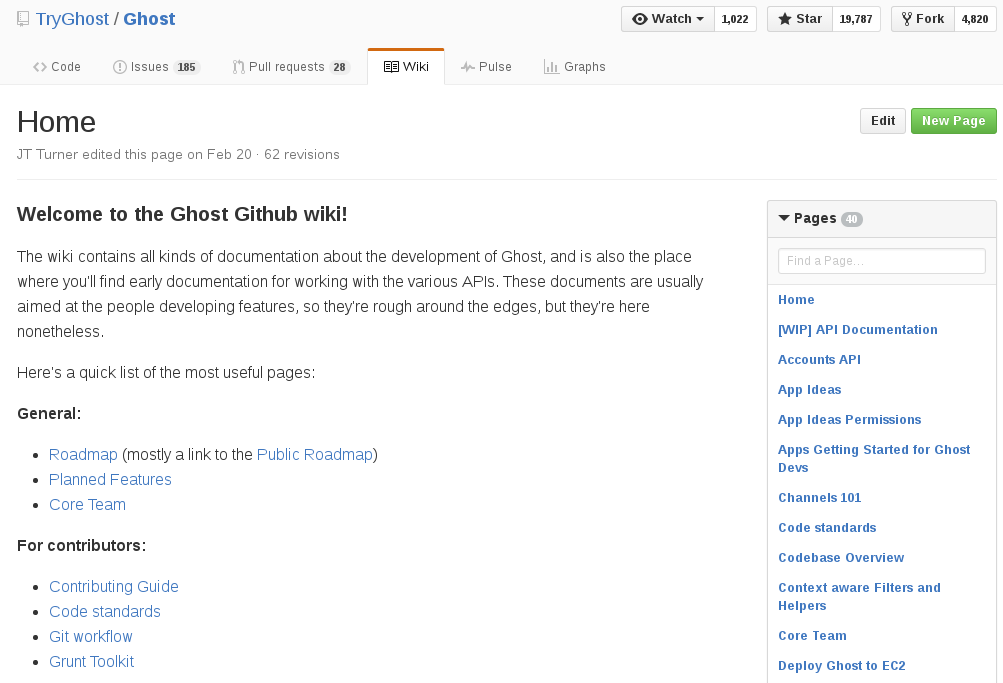
\includegraphics[height=12cm]{./assets/ghost3.png}
            \caption{Acceuil du wiki}
        \end{figure}

        Il est intéressant de constater les différences de stratégie de documentation des deux projets.
        D'un côté, Nylas N1 pousse la principe de la fusion des processus au maximum, en intégrant des
        paragraphes entiers de documentation au sein des commentaires de la source pour générer sa documentation.
        De l'autre, Ghost fait preuve d'une politique plus traditionnelle, en gardant une complètement séparé
        l'action de développer et celle de documenter. Il est possible de voir ici des raisons économiques,
        puisque Ghost est un projet actuellement beaucoup plus gros. Ainsi, les ressources humaines sont
        également plus importantes et permettent d'avoir un pouvoir de développement et la capacité de
        pouvoir documenter en même temps sans avoir à se poser de question. Mais cela peut aussi être
        le résultat d'un choix, où l'automatisation de la documentation demande une grande part de
        configuration et l'utilisation d'une multitude d'outils, ce qui compléxifie le développement.\\
        C'est sur base de ces observations que nous allons maintenant essayer de définir une stratégie
        de documentation pour le projet Buckless.


    \newpage
    \section{Application au projet Buckless}
        \subsection{Présentation du projet}
    \subsubsection{Contexte}
        \paragraph{}
            L’idée a vu le jour au sein de notre campus, en se basant sur des situations qui nous posaient problème.
            Vendre des produits ou des services peut être quelque chose de complexe si l’on considère le temps
            qu’il faut à un client pour accéder à un vendeur. De plus, ces derniers sont le plus souvent des étudiants
            volontaires qui n’ont pas l’expérience qu’un professionnel pourrait avoir, spécialement lors d’un rush.
            C’est pour cela que nous avons décidé de développer une solution de paiement entièrement dématérialisée
            pour optimiser les flux monétaires et logistiques lors des événements de notre école.

        \paragraph{}
            Buckless se démarque de certains projets similaires par le fait qu’il ne compte pas devenir un système
            de paiement global, intermédiaire de la banque. L’idée est de créer des monnaies locales, indépendantes
            entre chaque structure. Les clients gardent ainsi la main mise sur leur trésorerie et leur infrastructure
            informatique.
            La solution se présente sous la forme de bornes physiques (téléphones, tablettes, ordinateurs tactiles),
            utilisées par des vendeurs. Le client, lui, peut recharger un compte virtuel via une application en ligne,
            où via des points de rechargement physique directement sur site. Son moyen de paiement est défini par l'entreprise :
            un bracelet, un tatouage — pratique dans le monde événementiel — ou une carte — monde étudiant, ou encore
            son smartphone. Ce moyen de paiement permet d'identifier le client et de réaliser des achats instantanément.

    \subsubsection{Technologies utilisées}
        Le client de vente présent sur les bornes est une application web. En plus de l'avantage d'̂etre
        multi-plateforme, procéder ainsi permet le déploiement automatique de chaque nouvelle version
        du client sur les bornes. L'application web est entièrement écrite en javascript/css/html
        sous la forme d'une \textit{single page application}. Il a été choisi de construire le
        client à l'aide de \textit{Web Components}, une approche moderne et modulaire de développement.
        L'idée est de définir des composants indépendants, composés de leurs propres fichiers javascript/css/html,
        puis de les agencer afin d'obtenir l'application finale. Pour ce faire, le framework Vue.js
        a été choisi, bien que d'autres puissent faire de même (Angular.js, react, ..).\\
        Le serveur est développé en javascript sur la plateforme Node.js. Il est composé d'un service
        RESTful, de services d'authentification, et d'un serveur WebSocket pour la communication en
        temps réel.


\newpage
\subsection{Stratégie de documentation}
    \subsubsection
        A la vue des différents projets étudiés, de leurs approche de la documentationo, et des
        spécificités du projet Buckless, il a été possible de définir une stratégie de documentation.


    \subsubsection{UML - Diagrammes de composants}
        \paragraph{}
            Parmi la spécification d'UML, un type de diagramme sous-utilisé, le diagramme de composants,
            se révèle être un bon moyen de décrire les architectures utilisant des services.\\
            En effet, un service peut être vu comme un composant d'un système global, et les interfaces
            de ce composant comme les ressources exposées par le service.

        \paragraph{}
            L'approche "composant" au niveau logiciel est intéressante, car elle permet de rendre compte
            de l'architecture logicielle à une échelle plus grande que celle du diagramme de classe.
            Il est ainsi possible de modéliser les intéractions entre des grandes parties du logiciel,
            parties découpées de manière "fonctionnelle", et ce malgré d'éventuels changements au niveau
            du code.

        \begin{figure}[h]
            \centering
            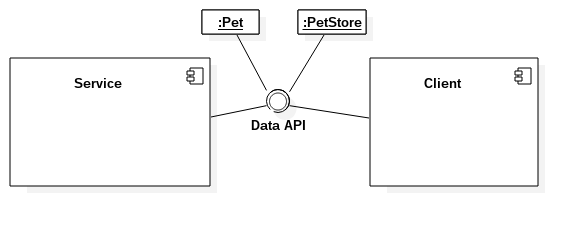
\includegraphics[scale=0.6]{./assets/UML/component1.png}
            \caption{Représentation avec des objets d'une API et ses ressources}
        \end{figure}

        \paragraph{}
            Un premier éssai de modélisation est donné ci-dessus. La première caractéristique d'une telle
            modélisation est l'impossibilité de voir où les ressources sont sollicitées au sein ̂meme
            du composant. De plus, à mesure que le nombre de ressource augmente,  l'encombrement visuel
            du à la représentation des instances passées rend la représentation difficile.

        \begin{figure}[h]
            \centering
            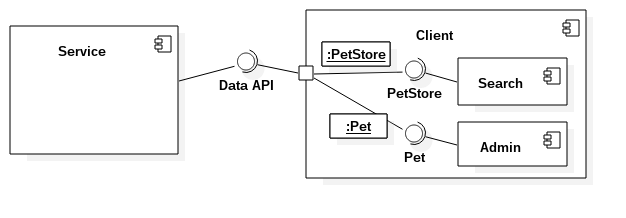
\includegraphics[scale=0.6]{./assets/UML/component3.png}
            \caption{Représentation d'une API et de ses ressources avec des interfaces}
        \end{figure}

        \paragraph{}
            La représentation de l'intéraction avec les sous composants (des WebComponent par exemple)
            est rendue possible par l'utilisation d'interfaces. De plus, pour éviter des diagrammes
            trop verbeux, on proposera la \textbf{convention} suivante pour les diagrammes de composants
            orientés service : \textbf{Une interface est homonyme au ressource qu'elle expose}.

        \begin{figure}[h]
            \centering
            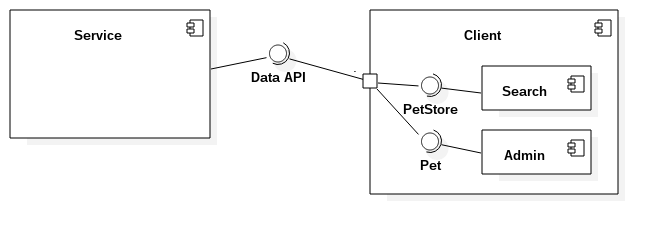
\includegraphics[scale=0.6]{./assets/UML/component2.png}
            \caption{Représentation d'une API et de ses ressources avec des interfaces homonymes aux instances}
        \end{figure}

        \paragraph{}
            Cette utilisation des interfaces renvoie directement à la définition (cf \ref{swaggerdef})
            du formalisme de description d'API Swagger. On remarque alors que le diagramme de composant pour
            les architectures orientées services, est aux formalismes de type Swagger ce que les diagrammes
            de classes sont aux commentaires de type Javadoc : une représentation visuelle alternative.

        \paragraph{}
            Il est intéressant de constater qu'il devient aisé d'avoir une vue globale de l'état
            d'utilisation des services (et donc des ressources) par les différentes parties de ou des
            logiciels. Un bénéfice immédiat de cette modélisation est donc de pouvoir anticiper l'impact
            qu'aurait la modification du fonctionnement d'un service, ou de la modification des modèles
            qui lui sont associés.

    \subsubsection{Représentation des modèles}
        La représentation au niveau composant de l'architecture logicelle a été jugée suffisamment
        détaillée pour ne pas descendre d'échelle et proposer des diagrammes de classes.\\
        En revanche, la question de pose de la représentation des différents modèles annotés en tant
        qu'interfaces sur le diagramme de composant. Pour cela, deux représentations possible :
        le diagramme entité / association (en notation UML ou notation de Chen), ou le diagramme de
        classes. Le premier offre une description d'un point de vue théorique, là ou le second se
        soucie des détails d'implémentations (description des tables de jointures, par exemple).
        Dans la mesure ou l'implémentation de la base de donnée n'a pas été prévue pour changer de
        technologie, il a été choisi de décrire cette dernière à l'aide de diagrammes de classes,
        complémentaires aux diagrammes de composants.

    \subsubsection{Description de l'API}
        Parallèlement au diagrammes de composants qui offrent une vue globale et visuelle des services
        (mais pas forcément exhaustive), nous avons du choisir un formalisme de type Swagger pour
        générer une documention dynamique de l'API.\\
        Le problème que nous avons eu avec Swagger est son principe déterministe\cite{determinism}.
        Il n'est pas possible de définir plusieurs blocs de réponses possible pour un même code http.
        Ainsi, nous avons du nous tourner vers une alternative : APIAry et la synthaxe Blueprint..

    \subsubsection{Commentaires et documentation}
        Nous avons vu au travers l'exemple de Nylas N1 qu'il était possible d'intégrer des larges
        portions de texte de documentation, dans l'optique de réunir code et documentation dans les
        même fichiers. Pour buckless, nous avons jugé cette pratique de vouloir réunir documentation
        et code un peu excessive, car parfois peu lisible au niveau du code source.
        C'est pourquoi nous nous sommes limités à des commentaires de types jsDoc simples.

    \subsubsection{Automatisation}
        Au niveau de l'automatisation de la production de la documentation, le duo linter et
        déploiement continu a été retenu. Pour des raisons de workflow incompatible (évoqué en
        \ref{hooks}), l'utilisation des hooks n'a pas été retenue.

\newpage
\subsection{Application pratique}
    Dans cette partie, nous essaierons de nous appuyer sur des éléments de documentations pratiques
    qui ont été produits pour le projet, afin de présenter certains mécanismes et choix techniques.
    Buckless étant un projet complexe, seul  les points les plus intéressants, ou les mieux représentés
    seront présentés ici.

    \subsubsection{Architecture globale}
        \begin{figure}[h]
            \centering
            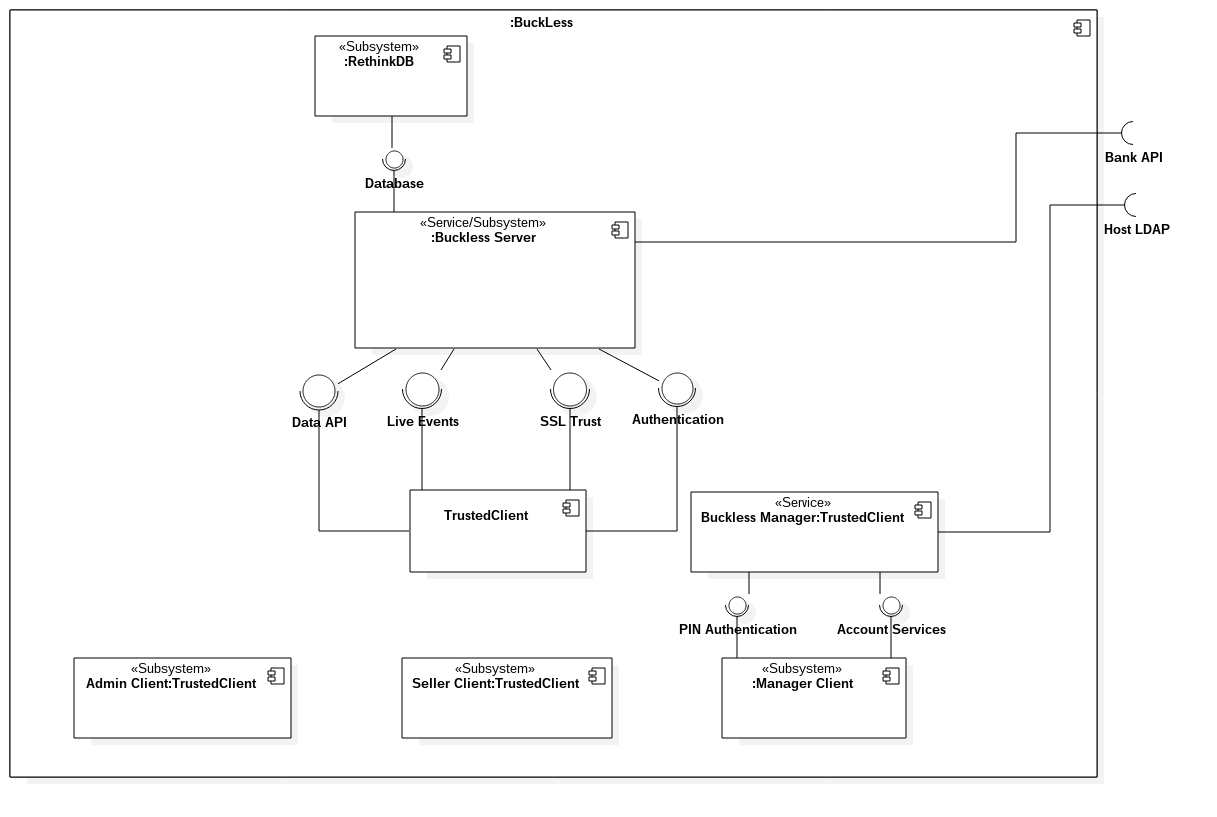
\includegraphics[height=12cm]{./assets/UML/system.png}
        \end{figure}

    \newpage
    \subsubsection{Architecture serveur}
        \begin{figure}[h]
            \centering
            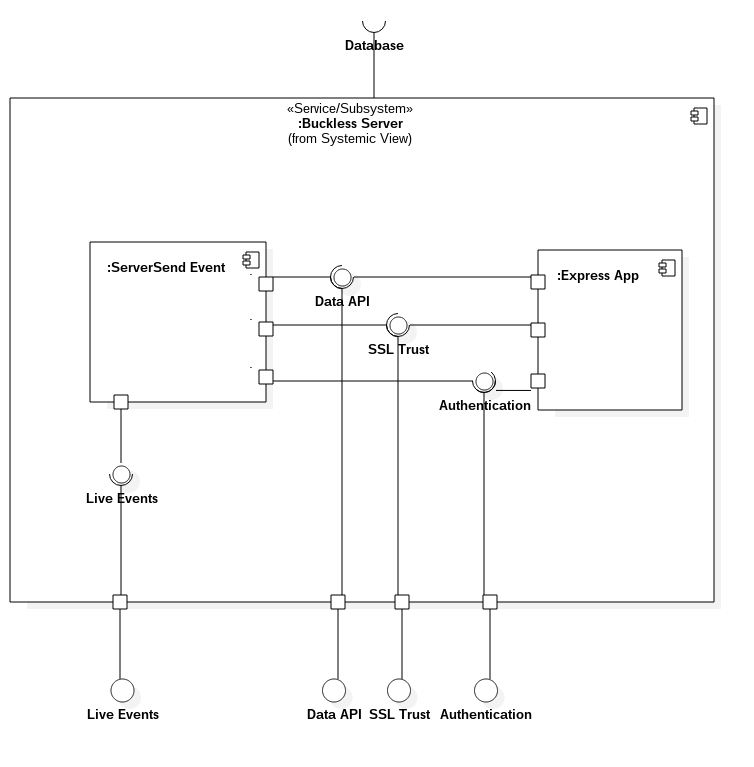
\includegraphics[height=12cm]{./assets/UML/buckless_server.png}
        \end{figure}

    \newpage
    \subsubsection{Architecture du client d'administration}
        \begin{figure}[h]
            \centering
            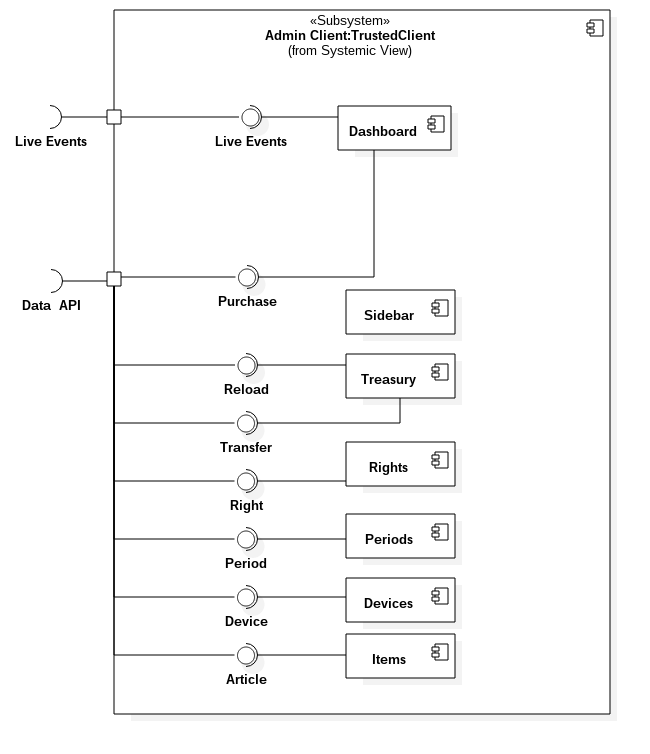
\includegraphics[height=12cm]{./assets/UML/admin_client.png}
        \end{figure}

    \newpage
    \subsubsection{Documentation dynamique de l'API}
        \begin{figure}[h]
            \centering
            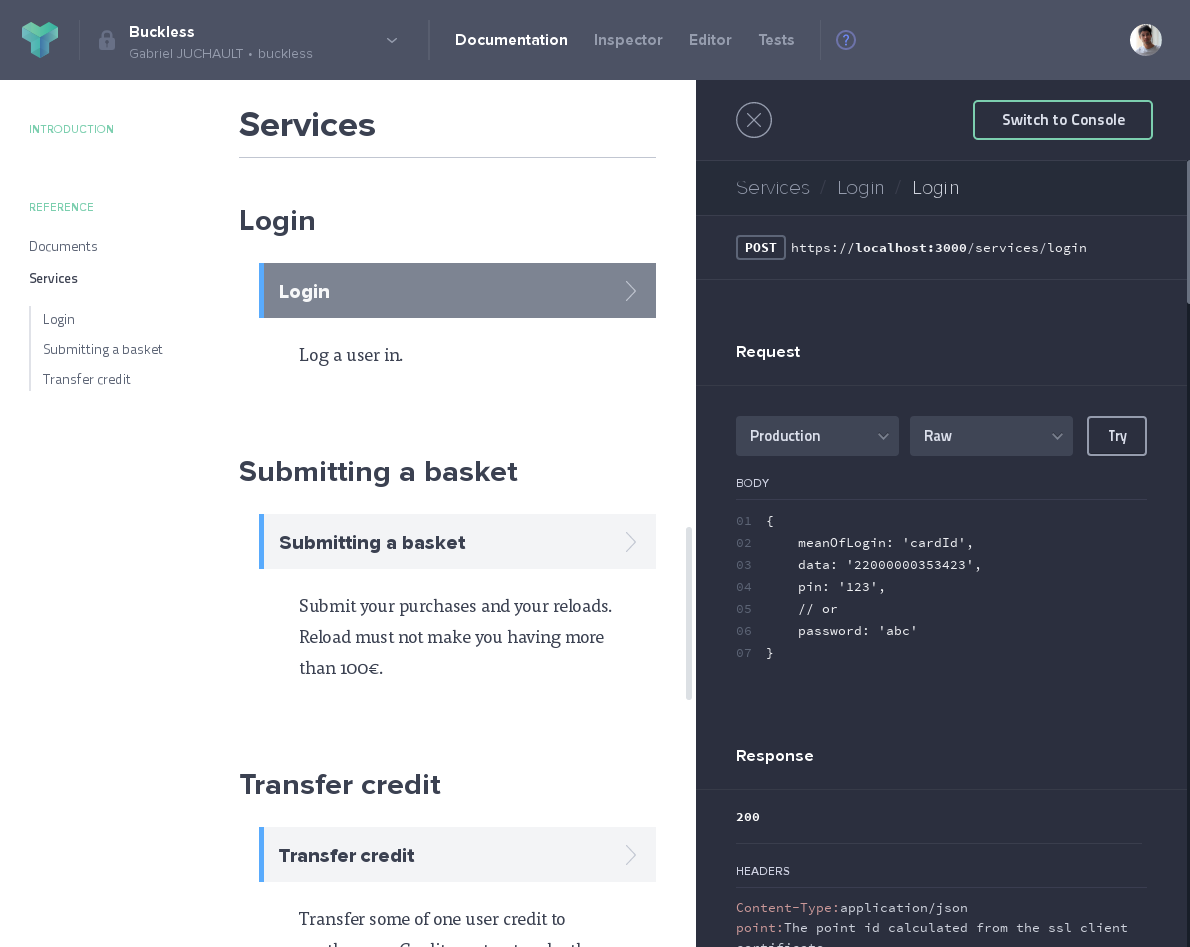
\includegraphics[height=12cm]{./assets/apiary.png}
        \end{figure}

    \newpage
    \section{Conclusion}
        \paragraph{}
    Aujourd'hui, il existe une grande diversité d'outils permettant de faciliter la production d'une
    documentation claire et complète. Nous avons vu qu'il était possible de faire en sorte d'automatiser
    un maximum l'utilisation de ces outils, afin de les intégrer au coeur du processus de développement
    logiciel.

\paragraph{}
    Le monde du logiciel libre est intimement lié avec la mise en oeuvre de stratégie de documentation
    efficace. En effet, l'attractivité du logiciel envers ses contributeurs est directement corrélé
    avec la présence d'une documentation complète minimisant le temps de formation.
    Au travers de l'exemple de Nylas, il a été force de constater que la documentation était au coeur
    de leur processus de développement. L'approche utilisée, consistant à l'automatisation à l'extrême
    par l'incorporation de la documentation au sein même du code, permet de lier le développeur
    inévitablement a une production de documentation.

\paragraph{}
    La définition d'une stratégie de documentation pour le projet Buckless a été faite en se basant
    sur les différents outils présentés dans l'état de l'art, mais aussi en prenant comme exemple
    des projets open source similaires comme Nylas N1. Il est cependant important de noter que malgré
    la simmilitude des projets au niveau technologique, certaines spécificités on fait que le modèle
    n'a pas pu être tout simplement calqué. Ainsi, il a été choisi d'explorer l'utilisation du
    diagramme de composants en tant qu'outil de représentation de système orienté service.
    L'intérêt de ce diagramme est double, puisqu'il permet de représenter à la fois les services
    web, mais aussi l'interaction des interne de chaque clients avec ces derniers.
    En effet, les technologies web se tournent de plus en plus vers l'utilisation de WebComponents
    réutilisables, appelant des services de manière indépendante. Il devient alors possible de représenter
    deux échelles d'un système sur un même diagramme. On regrette malheureusement l'absence d'outils
    permettant une intégration de la production de diagramme avec celle du code.

    \newpage
    \appendix
    \section{Diagrammes de composants}
\subsection{Ensemble des services}
    \begin{figure}[h]
        \centering
        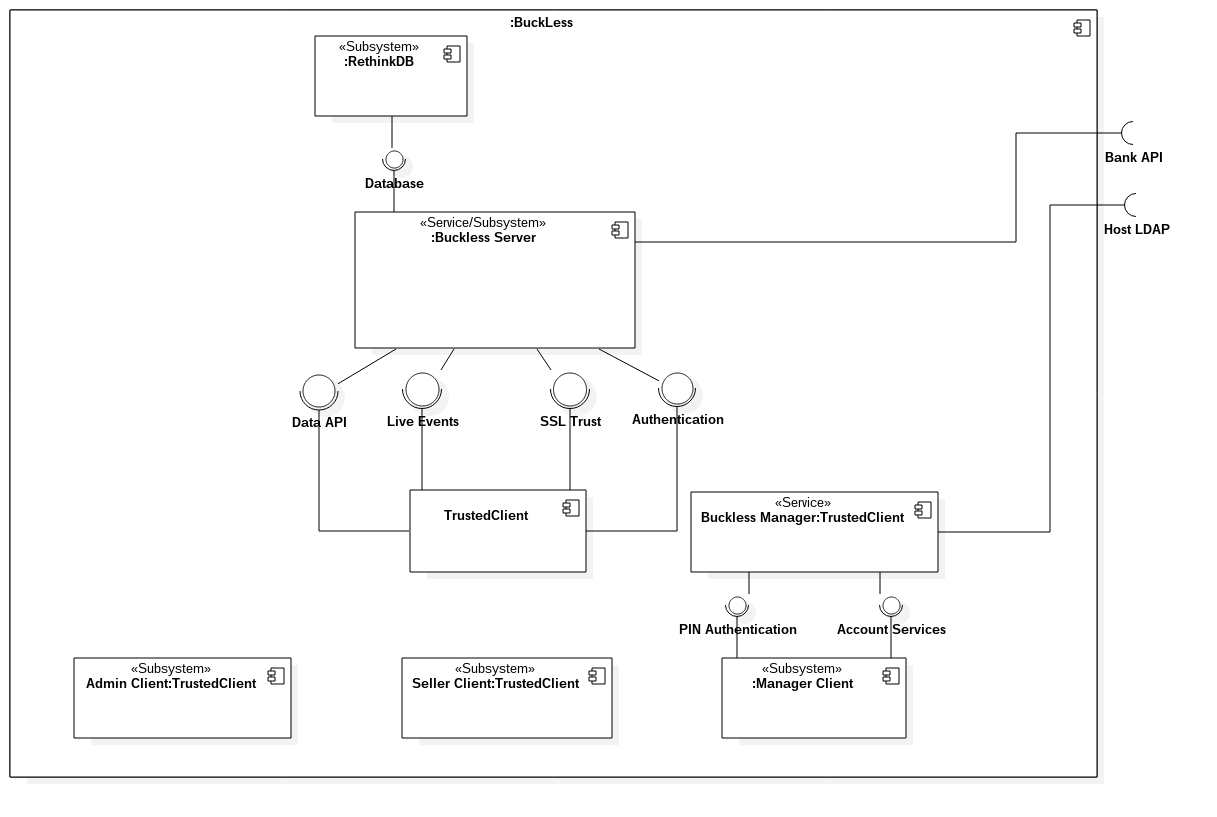
\includegraphics[scale=0.45]{./assets/UML/system.png}
        \label{system}
    \end{figure}

\newpage
\subsection{Structure interne du serveur}
    \begin{figure}[h]
        \centering
        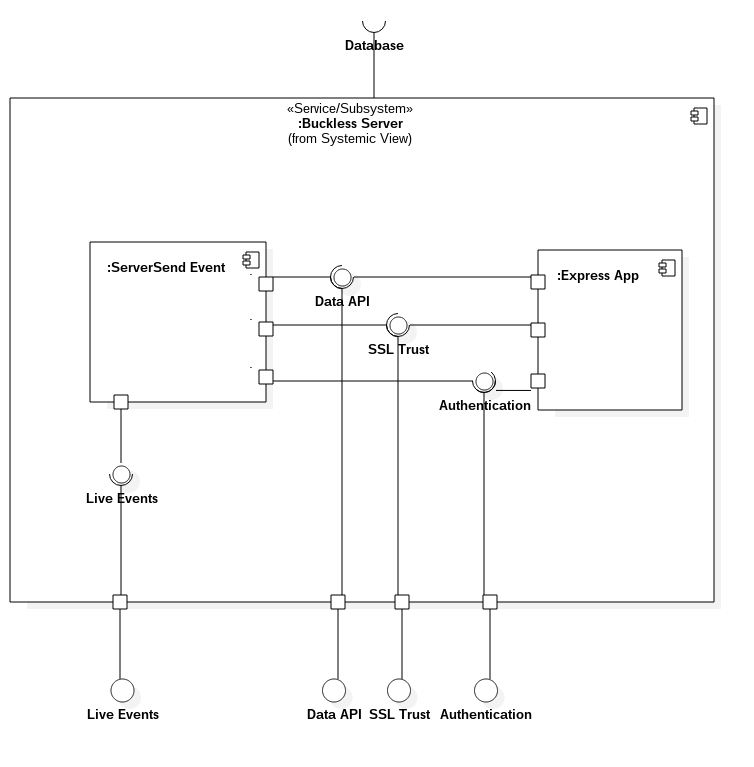
\includegraphics[scale=0.55]{./assets/UML/buckless_server.png}
        \label{buckless_server}
    \end{figure}

\newpage
\subsection{Structure interne du client d'administration}
    \begin{figure}[h]
        \centering
        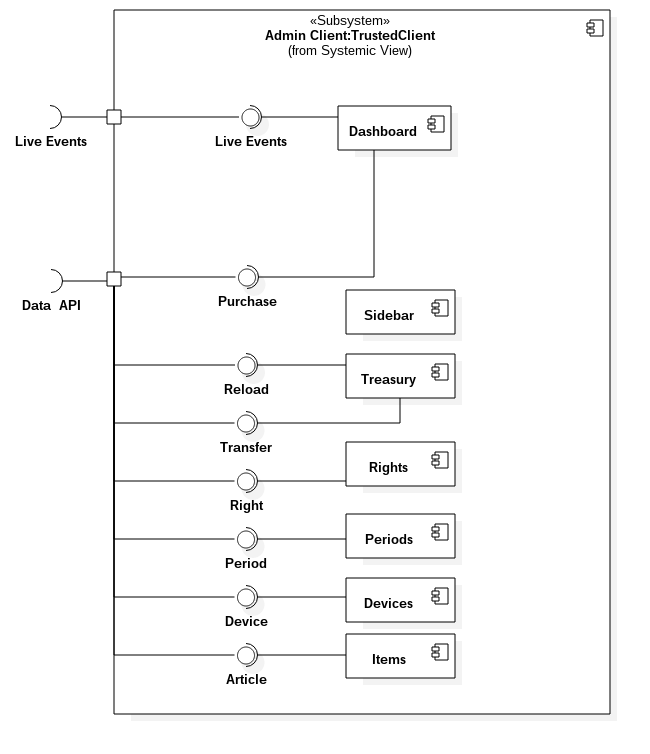
\includegraphics[scale=0.55]{./assets/UML/admin_client.png}
        \label{admin_client}
    \end{figure}

    \newpage
        \begin{thebibliography}{1}
            \bibitem{UML} UML 2 Component Diagrams: An Agile Introduction,
    \newblock Agile Modeling, \emph{Scott Ambler and Associates}\\
    \newblock \url{http://agilemodeling.com/artifacts/componentDiagram.htm}

\bibitem{UML2} The component diagram\\
    \newblock \url{http://www.ibm.com/developerworks/rational/library/dec04/bell/}

\bibitem{Swagger} Swagger, getting started\\
    \newblock \url{http://swagger.io/getting-started/}

\bibitem{SwaggerSpecs} Swagger, specifications\\
    \newblock \url{http://swagger.io/specification/}

\bibitem{wiki} Projects with great wikis,
    \newblock GitHub\\
    \newblock \url{https://github.com/showcases/projects-with-great-wikis}

\bibitem{tomdoc} TomDoc RFC\\
    \newblock \url{http://tomdoc.org/}

\bibitem{donna} Donna, A CoffeScript documentation generator,
    \newblock npmjs\\
    \newblock \url{https://www.npmjs.com/package/donna}

\bibitem{tello} Tello, Digests biscotto metadata,
    \newblock npmjs\\
    \newblock \url{https://www.npmjs.com/package/tello}
    \newblock \url{https://www.npmjs.com/package/donna}

\bibitem{ghpages} GitHub Pages, Websites for you and your projects,
    \newblock GitHub\\
    \newblock \url{https://pages.github.com/}
        \end{thebibliography}
\end{document}